\documentclass[12pt,a4paper]{article}
\usepackage[utf8]{inputenc}
\usepackage{amsmath}
\usepackage{amsfonts}
\usepackage{amssymb}
\usepackage[brazil]{babel}
\usepackage{indentfirst}
\usepackage{url}
\usepackage{float}
\usepackage{color}
\usepackage{tabela_de_dados}
\usepackage{tabela_de_dados_teste}
\usepackage{colortbl}

\definecolor{pblue}{rgb}{0.13,0.13,1}
\definecolor{pgreen}{rgb}{0,0.5,0}
\definecolor{pred}{rgb}{0.9,0,0}
\definecolor{pgrey}{rgb}{0.46,0.45,0.48}
\definecolor{cinzaClaro}{rgb}{0.9,0.9,0.9}

\definecolor{mygreen}{rgb}{0,0.6,0}
\definecolor{mygray}{rgb}{0.5,0.5,0.5}
\definecolor{mymauve}{rgb}{0.58,0,0.82}

\RequirePackage{graphicx}
\title{Dicionário de Dados}
\author{Gusttavo Nunes Gomes\and Jonathan Silvestre Sousa \and Salmi Nunes de Paula Junior\and Willian Wallace de Matteus Silva}
 
\usepackage[left=3cm,right=3cm,top=2cm,bottom=2cm]{geometry}
\begin{document}
\begin{titlepage}
\begin{center}
\begin{figure}[htb]
                
                \label{figura:LogoIF}
        
                \centering
                \includegraphics[width=6cm]{recursos/imagens/logo.png} 
\end{figure}
Instituto Federal Goiano - Campus Ceres\\
Bacharelado em Sistemas de Informação\\
Prof. Me. Ronneesley Moura Teles\\\vspace{1cm}

Gusttavo Nunes Gomes\\
Jonathan Silvestre Sousa \\
Salmi Nunes de Paula Junior\\
Willian Wallace de Matteus Silva\\
\vspace{6.0cm}
\textit{\textbf{\Large{Dicionário de Dados}}}\\\vspace{11cm}
Novembro\\
2017\\
\end{center}
\end{titlepage}
\tableofcontents
\newpage
\begin{center}
\textbf{\Large{Dicionário de Dados}}\\\vspace{0.5cm}
\end{center}
\section{Introdução}

\section{Dicionário de Dados - Rede Social}
\subsection{Eventos}

\begin{center}
\begin{table}[h!]
	\caption{\texttt{tipos\_atividades}}
	\label{tabela:tiposAtividades}
	%%%%%%%%%%%%%%%%%%%%Estrutura Tabela%%%%%%%%%%%%%%
	\begin{tabular}{|p{1cm}|p{1.5cm}|p{1.25cm}|p{1.25cm}|p{1.75cm}|p{1.25cm}|p{4.5cm}|}\hline	
		\multicolumn{7}{|p{16cm}|}{\cellcolor{cinzaClaro}  \centering Tabela: \texttt{tipos\_atividades}} \\ \hline %Parte superior da Tabela
		{\small Chaves} & {\small Campo Lógico} & {\small Campo Físico} & {\small Tipo} & {\small Tamanho} & {\small Nulo} & {\small Descrição}\\\hline %Parte com os nomes de cada Coluna
	%%%%%%%%%%%%%%%%%%%%Estrutura Tabela%%%%%%%%%%%%%%
		
		{\tiny } & {\tiny } & {\tiny } & {\tiny } & {\tiny } & {\tiny } &{\tiny }\\\hline
		{\tiny } & {\tiny } & {\tiny } & {\tiny } & {\tiny } & {\tiny } &{\tiny }\\\hline
		{\tiny } & {\tiny } & {\tiny } & {\tiny } & {\tiny } & {\tiny } &{\tiny }\\\hline
		
		%{\tiny } & {\tiny } & {\tiny } & {\tiny } & {\tiny } & {\tiny } &{\tiny }\\\hline %Modelo de novas linhas
			
	\end{tabular}
\end{table}	
\end{center}


\begin{center}
\begin{table}[h!]
	\caption{\texttt{atividades}}
	\label{tabela:atividades}
	%%%%%%%%%%%%%%%%%%%%Estrutura Tabela%%%%%%%%%%%%%%
	\begin{tabular}{|p{1cm}|p{1.5cm}|p{1.25cm}|p{1.25cm}|p{1.75cm}|p{1.25cm}|p{4.5cm}|}\hline	
		\multicolumn{7}{|p{16cm}|}{\cellcolor{cinzaClaro}  \centering Tabela: \texttt{atividades}} \\ \hline %Parte superior da Tabela
		{\small Chaves} & {\small Campo Lógico} & {\small Campo Físico} & {\small Tipo} & {\small Tamanho} & {\small Nulo} & {\small Descrição}\\\hline %Parte com os nomes de cada Coluna
	%%%%%%%%%%%%%%%%%%%%Estrutura Tabela%%%%%%%%%%%%%%
		
		{\tiny PK} & {\tiny Código} & {\tiny id} & {\tiny INT} & {\tiny } & {\tiny Not Null} &{\tiny Código da atividade.}\\\hline
		{\tiny } & {\tiny Nome} & {\tiny nome} & {\tiny VARCHAR} & {\tiny 100} & {\tiny Not Null} &{\tiny Nome da atividade.}\\\hline
		{\tiny } & {\tiny Descrição} & {\tiny descricao} & {\tiny TEXT} & {\tiny } & {\tiny Not Null} &{\tiny Descrição da atividade.}\\\hline
		{\tiny } & {\tiny Inicio} & {\tiny inicio} & {\tiny DATETIME} & {\tiny } & {\tiny Not Null} &{\tiny Data e hora de quando começará a atividade.}\\\hline
		{\tiny } & {\tiny Vagas} & {\tiny vagas} & {\tiny INT} & {\tiny } & {\tiny Null} &{\tiny Quantidade de vagas para essa atividade.}\\\hline
		{\tiny FK} & {\tiny Evento} & {\tiny evento} & {\tiny INT} & {\tiny } & {\tiny Not Null} &{\tiny Código do evento vinculado.}\\\hline
		{\tiny FK} & {\tiny Tipo de atividade} & {\tiny tipo} & {\tiny INT} & {\tiny } & {\tiny Not Null} &{\tiny Código do tipo de atividade vinculado.}\\\hline
		
		%{\tiny ID} & {\tiny ID} & {\tiny ID} & {\tiny ID} & {\tiny ID} & {\tiny ID} &{\tiny ID}\\\hline %Modelo de novas linhas
			
	\end{tabular}
\end{table}	
\end{center}


\begin{center}
\begin{table}[h!]
	\caption{\texttt{presenca\_atividades}}
	\label{tabela:presencaAtividades}
	%%%%%%%%%%%%%%%%%%%%Estrutura Tabela%%%%%%%%%%%%%%
	\begin{tabular}{|p{1cm}|p{1.5cm}|p{1.25cm}|p{1.25cm}|p{1.75cm}|p{1.25cm}|p{4.5cm}|}\hline	
		\multicolumn{7}{|p{16cm}|}{\cellcolor{cinzaClaro}  \centering Tabela: \texttt{presenca\_atividades}} \\ \hline %Parte superior da Tabela
		{\small Chaves} & {\small Campo Lógico} & {\small Campo Físico} & {\small Tipo} & {\small Tamanho} & {\small Nulo} & {\small Descrição}\\\hline %Parte com os nomes de cada Coluna
	%%%%%%%%%%%%%%%%%%%%Estrutura Tabela%%%%%%%%%%%%%%
		
		{\tiny } & {\tiny } & {\tiny } & {\tiny } & {\tiny } & {\tiny } &{\tiny }\\\hline
		{\tiny } & {\tiny } & {\tiny } & {\tiny } & {\tiny } & {\tiny } &{\tiny }\\\hline
		{\tiny } & {\tiny } & {\tiny } & {\tiny } & {\tiny } & {\tiny } &{\tiny }\\\hline
		
		%{\tiny } & {\tiny } & {\tiny } & {\tiny } & {\tiny } & {\tiny } &{\tiny }\\\hline %Modelo de novas linhas
			
	\end{tabular}
\end{table}	
\end{center}


\begin{center}
\begin{table}[h!]
	\caption{\texttt{responsaveis\_atividades}}
	\label{tabela:responsaveisAtividades}
	%%%%%%%%%%%%%%%%%%%%Estrutura Tabela%%%%%%%%%%%%%%
	\begin{tabular}{|p{1cm}|p{1.5cm}|p{1.25cm}|p{1.25cm}|p{1.75cm}|p{1.25cm}|p{4.5cm}|}\hline	
		\multicolumn{7}{|p{16cm}|}{\cellcolor{cinzaClaro}  \centering Tabela: \texttt{responsaveis\_atividades}} \\ \hline %Parte superior da Tabela
		{\small Chaves} & {\small Campo Lógico} & {\small Campo Físico} & {\small Tipo} & {\small Tamanho} & {\small Nulo} & {\small Descrição}\\\hline %Parte com os nomes de cada Coluna
	%%%%%%%%%%%%%%%%%%%%Estrutura Tabela%%%%%%%%%%%%%%
		
		{\tiny } & {\tiny } & {\tiny } & {\tiny } & {\tiny } & {\tiny } &{\tiny }\\\hline
		{\tiny } & {\tiny } & {\tiny } & {\tiny } & {\tiny } & {\tiny } &{\tiny }\\\hline
		{\tiny } & {\tiny } & {\tiny } & {\tiny } & {\tiny } & {\tiny } &{\tiny }\\\hline
		
		%{\tiny } & {\tiny } & {\tiny } & {\tiny } & {\tiny } & {\tiny } &{\tiny }\\\hline %Modelo de novas linhas
			
	\end{tabular}
\end{table}	
\end{center}


\begin{center}
\begin{table}[h!]
	\caption{\texttt{organizadores\_eventos}}
	\label{tabela:organizadoresEventos}
	%%%%%%%%%%%%%%%%%%%%Estrutura Tabela%%%%%%%%%%%%%%
	\begin{tabular}{|p{1cm}|p{1.5cm}|p{1.25cm}|p{1.25cm}|p{1.75cm}|p{1.25cm}|p{4.5cm}|}\hline	
		\multicolumn{7}{|p{16cm}|}{\cellcolor{cinzaClaro}  \centering Tabela: \texttt{organizadores\_eventos}} \\ \hline %Parte superior da Tabela
		{\small Chaves} & {\small Campo Lógico} & {\small Campo Físico} & {\small Tipo} & {\small Tamanho} & {\small Nulo} & {\small Descrição}\\\hline %Parte com os nomes de cada Coluna
	%%%%%%%%%%%%%%%%%%%%Estrutura Tabela%%%%%%%%%%%%%%
		
		{\tiny } & {\tiny } & {\tiny } & {\tiny } & {\tiny } & {\tiny } &{\tiny }\\\hline
		{\tiny } & {\tiny } & {\tiny } & {\tiny } & {\tiny } & {\tiny } &{\tiny }\\\hline
		
		%{\tiny } & {\tiny } & {\tiny } & {\tiny } & {\tiny } & {\tiny } &{\tiny }\\\hline %Modelo de novas linhas
			
	\end{tabular}
\end{table}	
\end{center}


\begin{center}
\begin{table}[h!]
	\caption{\texttt{presenca\_evento}}
	\label{tabela:presencaEvento}
	%%%%%%%%%%%%%%%%%%%%Estrutura Tabela%%%%%%%%%%%%%%
	\begin{tabular}{|p{1cm}|p{1.5cm}|p{1.25cm}|p{1.25cm}|p{1.75cm}|p{1.25cm}|p{4.5cm}|}\hline	
		\multicolumn{7}{|p{16cm}|}{\cellcolor{cinzaClaro}  \centering Tabela: \texttt{presenca\_evento}} \\ \hline %Parte superior da Tabela
		{\small Chaves} & {\small Campo Lógico} & {\small Campo Físico} & {\small Tipo} & {\small Tamanho} & {\small Nulo} & {\small Descrição}\\\hline %Parte com os nomes de cada Coluna
	%%%%%%%%%%%%%%%%%%%%Estrutura Tabela%%%%%%%%%%%%%%
		
		{\tiny } & {\tiny } & {\tiny } & {\tiny } & {\tiny } & {\tiny } &{\tiny }\\\hline
		{\tiny } & {\tiny } & {\tiny } & {\tiny } & {\tiny } & {\tiny } &{\tiny }\\\hline
		
		%{\tiny } & {\tiny } & {\tiny } & {\tiny } & {\tiny } & {\tiny } &{\tiny }\\\hline %Modelo de novas linhas
			
	\end{tabular}
\end{table}	
\end{center}


\begin{center}
\begin{table}[h!]
	\caption{\texttt{eventos}}
	\label{tabela:eventos}
	%%%%%%%%%%%%%%%%%%%%Estrutura Tabela%%%%%%%%%%%%%%
	\begin{tabular}{|p{1cm}|p{1.5cm}|p{1.25cm}|p{1.25cm}|p{1.75cm}|p{1.25cm}|p{4.5cm}|}\hline	
		\multicolumn{7}{|p{16cm}|}{\cellcolor{cinzaClaro}  \centering Tabela: \texttt{eventos}} \\ \hline %Parte superior da Tabela
		{\small Chaves} & {\small Campo Lógico} & {\small Campo Físico} & {\small Tipo} & {\small Tamanho} & {\small Nulo} & {\small Descrição}\\\hline %Parte com os nomes de cada Coluna
	%%%%%%%%%%%%%%%%%%%%Estrutura Tabela%%%%%%%%%%%%%%
		
		{\tiny } & {\tiny } & {\tiny } & {\tiny } & {\tiny } & {\tiny } &{\tiny }\\\hline
		{\tiny } & {\tiny } & {\tiny } & {\tiny } & {\tiny } & {\tiny } &{\tiny }\\\hline
		{\tiny } & {\tiny } & {\tiny } & {\tiny } & {\tiny } & {\tiny } &{\tiny }\\\hline
		{\tiny } & {\tiny } & {\tiny } & {\tiny } & {\tiny } & {\tiny } &{\tiny }\\\hline
		{\tiny } & {\tiny } & {\tiny } & {\tiny } & {\tiny } & {\tiny } &{\tiny }\\\hline
		{\tiny } & {\tiny } & {\tiny } & {\tiny } & {\tiny } & {\tiny } &{\tiny }\\\hline
		{\tiny } & {\tiny } & {\tiny } & {\tiny } & {\tiny } & {\tiny } &{\tiny }\\\hline
		{\tiny } & {\tiny } & {\tiny } & {\tiny } & {\tiny } & {\tiny } &{\tiny }\\\hline
		{\tiny } & {\tiny } & {\tiny } & {\tiny } & {\tiny } & {\tiny } &{\tiny }\\\hline
		
		%{\tiny } & {\tiny } & {\tiny } & {\tiny } & {\tiny } & {\tiny } &{\tiny }\\\hline %Modelo de novas linhas
			
	\end{tabular}
\end{table}	
\end{center}

\subsection{Artefatos do usuários}

%Inserir as tabelas de Artefatos do usuários

\begin{center}
\begin{table}[h!]
	\caption{\texttt{usuarios}}
	\label{tabela:usuarios}
	%%%%%%%%%%%%%%%%%%%%Estrutura Tabela%%%%%%%%%%%%%%
	\begin{tabular}{|p{1cm}|p{1.5cm}|p{1.25cm}|p{1.25cm}|p{1.75cm}|p{1.25cm}|p{4.5cm}|}\hline	
		\multicolumn{7}{|p{16cm}|}{\cellcolor{cinzaClaro}  \centering Tabela: \texttt{usuarios}} \\ \hline %Parte superior da Tabela
		{\small Chaves} & {\small Campo Lógico} & {\small Campo Físico} & {\small Tipo} & {\small Tamanho} & {\small Nulo} & {\small Descrição}\\\hline %Parte com os nomes de cada Coluna
	%%%%%%%%%%%%%%%%%%%%Estrutura Tabela%%%%%%%%%%%%%%
		
		{\tiny } & {\tiny } & {\tiny } & {\tiny } & {\tiny } & {\tiny } &{\tiny }\\\hline
		{\tiny } & {\tiny } & {\tiny } & {\tiny } & {\tiny } & {\tiny } &{\tiny }\\\hline
		{\tiny } & {\tiny } & {\tiny } & {\tiny } & {\tiny } & {\tiny } &{\tiny }\\\hline
		{\tiny } & {\tiny } & {\tiny } & {\tiny } & {\tiny } & {\tiny } &{\tiny }\\\hline
		{\tiny } & {\tiny } & {\tiny } & {\tiny } & {\tiny } & {\tiny } &{\tiny }\\\hline
		{\tiny } & {\tiny } & {\tiny } & {\tiny } & {\tiny } & {\tiny } &{\tiny }\\\hline
		{\tiny } & {\tiny } & {\tiny } & {\tiny } & {\tiny } & {\tiny } &{\tiny }\\\hline
		{\tiny } & {\tiny } & {\tiny } & {\tiny } & {\tiny } & {\tiny } &{\tiny }\\\hline
		{\tiny } & {\tiny } & {\tiny } & {\tiny } & {\tiny } & {\tiny } &{\tiny }\\\hline		
		{\tiny } & {\tiny } & {\tiny } & {\tiny } & {\tiny } & {\tiny } &{\tiny }\\\hline
		{\tiny } & {\tiny } & {\tiny } & {\tiny } & {\tiny } & {\tiny } &{\tiny }\\\hline
		
		%{\tiny } & {\tiny } & {\tiny } & {\tiny } & {\tiny } & {\tiny } &{\tiny }\\\hline %Modelo de novas linhas
			
	\end{tabular}
\end{table}	
\end{center}



\begin{center}
\begin{table}[h!]
	\caption{\texttt{relacionamentos}}
	\label{tabela:relacionamentos}
	%%%%%%%%%%%%%%%%%%%%Estrutura Tabela%%%%%%%%%%%%%%
	\begin{tabular}{|p{1cm}|p{1.5cm}|p{1.25cm}|p{1.25cm}|p{1.75cm}|p{1.25cm}|p{4.5cm}|}\hline	
		\multicolumn{7}{|p{16cm}|}{\cellcolor{cinzaClaro}  \centering Tabela: \texttt{relacionamentos}} \\ \hline %Parte superior da Tabela
		{\small Chaves} & {\small Campo Lógico} & {\small Campo Físico} & {\small Tipo} & {\small Tamanho} & {\small Nulo} & {\small Descrição}\\\hline %Parte com os nomes de cada Coluna
	%%%%%%%%%%%%%%%%%%%%Estrutura Tabela%%%%%%%%%%%%%%
		
		{\tiny } & {\tiny } & {\tiny } & {\tiny } & {\tiny } & {\tiny } &{\tiny }\\\hline
		{\tiny } & {\tiny } & {\tiny } & {\tiny } & {\tiny } & {\tiny } &{\tiny }\\\hline
		{\tiny } & {\tiny } & {\tiny } & {\tiny } & {\tiny } & {\tiny } &{\tiny }\\\hline
		
		%{\tiny } & {\tiny } & {\tiny } & {\tiny } & {\tiny } & {\tiny } &{\tiny }\\\hline %Modelo de novas linhas
			
	\end{tabular}
\end{table}	
\end{center}

\begin{center}
\begin{table}[h!]
	\caption{\texttt{autores}}
	\label{tabela:autores}
	%%%%%%%%%%%%%%%%%%%%Estrutura Tabela%%%%%%%%%%%%%%
	\begin{tabular}{|p{1cm}|p{1.5cm}|p{1.25cm}|p{1.25cm}|p{1.75cm}|p{1.25cm}|p{4.5cm}|}\hline	
		\multicolumn{7}{|p{16cm}|}{\cellcolor{cinzaClaro}  \centering Tabela: \texttt{autores}} \\ \hline %Parte superior da Tabela
		{\small Chaves} & {\small Campo Lógico} & {\small Campo Físico} & {\small Tipo} & {\small Tamanho} & {\small Nulo} & {\small Descrição}\\\hline %Parte com os nomes de cada Coluna
	%%%%%%%%%%%%%%%%%%%%Estrutura Tabela%%%%%%%%%%%%%%
		
		{\tiny } & {\tiny } & {\tiny } & {\tiny } & {\tiny } & {\tiny } &{\tiny }\\\hline
		{\tiny } & {\tiny } & {\tiny } & {\tiny } & {\tiny } & {\tiny } &{\tiny }\\\hline
		
		%{\tiny } & {\tiny } & {\tiny } & {\tiny } & {\tiny } & {\tiny } &{\tiny }\\\hline %Modelo de novas linhas
			
	\end{tabular}
\end{table}	
\end{center}





\begin{center}
\begin{table}[h!]
	\caption{\texttt{albuns}}
	\label{tabela:albuns}
	%%%%%%%%%%%%%%%%%%%%Estrutura Tabela%%%%%%%%%%%%%%
	\begin{tabular}{|p{1cm}|p{1.5cm}|p{1.25cm}|p{1.25cm}|p{1.75cm}|p{1.25cm}|p{4.5cm}|}\hline	
		\multicolumn{7}{|p{16cm}|}{\cellcolor{cinzaClaro}  \centering Tabela: \texttt{albuns}} \\ \hline %Parte superior da Tabela
		{\small Chaves} & {\small Campo Lógico} & {\small Campo Físico} & {\small Tipo} & {\small Tamanho} & {\small Nulo} & {\small Descrição}\\\hline %Parte com os nomes de cada Coluna
	%%%%%%%%%%%%%%%%%%%%Estrutura Tabela%%%%%%%%%%%%%%
		
		{\tiny } & {\tiny } & {\tiny } & {\tiny } & {\tiny } & {\tiny } &{\tiny }\\\hline
		{\tiny } & {\tiny } & {\tiny } & {\tiny } & {\tiny } & {\tiny } &{\tiny }\\\hline
		{\tiny } & {\tiny } & {\tiny } & {\tiny } & {\tiny } & {\tiny } &{\tiny }\\\hline
		{\tiny } & {\tiny } & {\tiny } & {\tiny } & {\tiny } & {\tiny } &{\tiny }\\\hline
		
		%{\tiny } & {\tiny } & {\tiny } & {\tiny } & {\tiny } & {\tiny } &{\tiny }\\\hline %Modelo de novas linhas
			
	\end{tabular}
\end{table}	
\end{center}


\begin{center}
\begin{table}[h!]
	\caption{\texttt{multimidias}}
	\label{tabela:multimidias}
	%%%%%%%%%%%%%%%%%%%%Estrutura Tabela%%%%%%%%%%%%%%
	\begin{tabular}{|p{1cm}|p{1.5cm}|p{1.25cm}|p{1.25cm}|p{1.75cm}|p{1.25cm}|p{4.5cm}|}\hline	
		\multicolumn{7}{|p{16cm}|}{\cellcolor{cinzaClaro}  \centering Tabela: \texttt{multimidias}} \\ \hline %Parte superior da Tabela
		{\small Chaves} & {\small Campo Lógico} & {\small Campo Físico} & {\small Tipo} & {\small Tamanho} & {\small Nulo} & {\small Descrição}\\\hline %Parte com os nomes de cada Coluna
	%%%%%%%%%%%%%%%%%%%%Estrutura Tabela%%%%%%%%%%%%%%
		
		{\tiny } & {\tiny } & {\tiny } & {\tiny } & {\tiny } & {\tiny } &{\tiny }\\\hline
		{\tiny } & {\tiny } & {\tiny } & {\tiny } & {\tiny } & {\tiny } &{\tiny }\\\hline
		{\tiny } & {\tiny } & {\tiny } & {\tiny } & {\tiny } & {\tiny } &{\tiny }\\\hline
		{\tiny } & {\tiny } & {\tiny } & {\tiny } & {\tiny } & {\tiny } &{\tiny }\\\hline
		{\tiny } & {\tiny } & {\tiny } & {\tiny } & {\tiny } & {\tiny } &{\tiny }\\\hline
		
		%{\tiny } & {\tiny } & {\tiny } & {\tiny } & {\tiny } & {\tiny } &{\tiny }\\\hline %Modelo de novas linhas
			
	\end{tabular}
\end{table}	
\end{center}

\subsection{Postagens}

%Inserir as tabelas de Postagens

\begin{center}
\begin{table}[h!]
	\caption{\texttt{categorias}}
	\label{tabela:categorias}
	%%%%%%%%%%%%%%%%%%%%Estrutura Tabela%%%%%%%%%%%%%%
	\begin{tabular}{|p{1cm}|p{1.5cm}|p{1.25cm}|p{1.25cm}|p{1.75cm}|p{1.25cm}|p{4.5cm}|}\hline	
		\multicolumn{7}{|p{16cm}|}{\cellcolor{cinzaClaro}  \centering Tabela: \texttt{categorias}} \\ \hline %Parte superior da Tabela
		{\small Chaves} & {\small Campo Lógico} & {\small Campo Físico} & {\small Tipo} & {\small Tamanho} & {\small Nulo} & {\small Descrição}\\\hline %Parte com os nomes de cada Coluna
	%%%%%%%%%%%%%%%%%%%%Estrutura Tabela%%%%%%%%%%%%%%
		
		{\tiny } & {\tiny } & {\tiny } & {\tiny } & {\tiny } & {\tiny } &{\tiny }\\\hline
		{\tiny } & {\tiny } & {\tiny } & {\tiny } & {\tiny } & {\tiny } &{\tiny }\\\hline
		
		%{\tiny } & {\tiny } & {\tiny } & {\tiny } & {\tiny } & {\tiny } &{\tiny }\\\hline %Modelo de novas linhas
			
	\end{tabular}
\end{table}	
\end{center}

\begin{center}
\begin{table}[h!]
	\caption{\texttt{aportes}}
	\label{tabela:aportes}
	%%%%%%%%%%%%%%%%%%%%Estrutura Tabela%%%%%%%%%%%%%%
	\begin{tabular}{|p{1cm}|p{1.5cm}|p{1.25cm}|p{1.25cm}|p{1.75cm}|p{1.25cm}|p{4.5cm}|}\hline	
		\multicolumn{7}{|p{16cm}|}{\cellcolor{cinzaClaro}  \centering Tabela: \texttt{aportes}} \\ \hline %Parte superior da Tabela
		{\small Chaves} & {\small Campo Lógico} & {\small Campo Físico} & {\small Tipo} & {\small Tamanho} & {\small Nulo} & {\small Descrição}\\\hline %Parte com os nomes de cada Coluna
	%%%%%%%%%%%%%%%%%%%%Estrutura Tabela%%%%%%%%%%%%%%
		
		{\tiny } & {\tiny } & {\tiny } & {\tiny } & {\tiny } & {\tiny } &{\tiny }\\\hline
		{\tiny } & {\tiny } & {\tiny } & {\tiny } & {\tiny } & {\tiny } &{\tiny }\\\hline
		{\tiny } & {\tiny } & {\tiny } & {\tiny } & {\tiny } & {\tiny } &{\tiny }\\\hline
		{\tiny } & {\tiny } & {\tiny } & {\tiny } & {\tiny } & {\tiny } &{\tiny }\\\hline
		
		%{\tiny } & {\tiny } & {\tiny } & {\tiny } & {\tiny } & {\tiny } &{\tiny }\\\hline %Modelo de novas linhas
			
	\end{tabular}
\end{table}	
\end{center}

\begin{center}
\begin{table}[h!]
	\caption{\texttt{postagens}}
	\label{tabela:postagens}
	%%%%%%%%%%%%%%%%%%%%Estrutura Tabela%%%%%%%%%%%%%%
	\begin{tabular}{|p{1cm}|p{1.5cm}|p{1.25cm}|p{1.25cm}|p{1.75cm}|p{1.25cm}|p{4.5cm}|}\hline	
		\multicolumn{7}{|p{16cm}|}{\cellcolor{cinzaClaro}  \centering Tabela: \texttt{postagens}} \\ \hline %Parte superior da Tabela
		{\small Chaves} & {\small Campo Lógico} & {\small Campo Físico} & {\small Tipo} & {\small Tamanho} & {\small Nulo} & {\small Descrição}\\\hline %Parte com os nomes de cada Coluna
	%%%%%%%%%%%%%%%%%%%%Estrutura Tabela%%%%%%%%%%%%%%
		
		{\tiny } & {\tiny } & {\tiny } & {\tiny } & {\tiny } & {\tiny } &{\tiny }\\\hline
		{\tiny } & {\tiny } & {\tiny } & {\tiny } & {\tiny } & {\tiny } &{\tiny }\\\hline
		{\tiny } & {\tiny } & {\tiny } & {\tiny } & {\tiny } & {\tiny } &{\tiny }\\\hline
		{\tiny } & {\tiny } & {\tiny } & {\tiny } & {\tiny } & {\tiny } &{\tiny }\\\hline
		{\tiny } & {\tiny } & {\tiny } & {\tiny } & {\tiny } & {\tiny } &{\tiny }\\\hline
		{\tiny } & {\tiny } & {\tiny } & {\tiny } & {\tiny } & {\tiny } &{\tiny }\\\hline
		{\tiny } & {\tiny } & {\tiny } & {\tiny } & {\tiny } & {\tiny } &{\tiny }\\\hline
		
		%{\tiny } & {\tiny } & {\tiny } & {\tiny } & {\tiny } & {\tiny } &{\tiny }\\\hline %Modelo de novas linhas
			
	\end{tabular}
\end{table}	
\end{center}

\begin{center}
\begin{table}[h!]
	\caption{\texttt{comentarios}}
	\label{tabela:comentarios}
	%%%%%%%%%%%%%%%%%%%%Estrutura Tabela%%%%%%%%%%%%%%
	\begin{tabular}{|p{1cm}|p{1.5cm}|p{1.25cm}|p{1.25cm}|p{1.75cm}|p{1.25cm}|p{4.5cm}|}\hline	
		\multicolumn{7}{|p{16cm}|}{\cellcolor{cinzaClaro}  \centering Tabela: \texttt{comentarios}} \\ \hline %Parte superior da Tabela
		{\small Chaves} & {\small Campo Lógico} & {\small Campo Físico} & {\small Tipo} & {\small Tamanho} & {\small Nulo} & {\small Descrição}\\\hline %Parte com os nomes de cada Coluna
	%%%%%%%%%%%%%%%%%%%%Estrutura Tabela%%%%%%%%%%%%%%
		
		{\tiny } & {\tiny } & {\tiny } & {\tiny } & {\tiny } & {\tiny } &{\tiny }\\\hline
		{\tiny } & {\tiny } & {\tiny } & {\tiny } & {\tiny } & {\tiny } &{\tiny }\\\hline
		{\tiny } & {\tiny } & {\tiny } & {\tiny } & {\tiny } & {\tiny } &{\tiny }\\\hline
		{\tiny } & {\tiny } & {\tiny } & {\tiny } & {\tiny } & {\tiny } &{\tiny }\\\hline
		{\tiny } & {\tiny } & {\tiny } & {\tiny } & {\tiny } & {\tiny } &{\tiny }\\\hline
		{\tiny } & {\tiny } & {\tiny } & {\tiny } & {\tiny } & {\tiny } &{\tiny }\\\hline
		{\tiny } & {\tiny } & {\tiny } & {\tiny } & {\tiny } & {\tiny } &{\tiny }\\\hline
		{\tiny } & {\tiny } & {\tiny } & {\tiny } & {\tiny } & {\tiny } &{\tiny }\\\hline
		
		%{\tiny } & {\tiny } & {\tiny } & {\tiny } & {\tiny } & {\tiny } &{\tiny }\\\hline %Modelo de novas linhas
			
	\end{tabular}
\end{table}	
\end{center}

\begin{center}
\begin{table}[h!]
	\caption{\texttt{palavras\_chave}}
	\label{tabela:palavrasChave}
	%%%%%%%%%%%%%%%%%%%%Estrutura Tabela%%%%%%%%%%%%%%
	\begin{tabular}{|p{1cm}|p{1.5cm}|p{1.25cm}|p{1.25cm}|p{1.75cm}|p{1.25cm}|p{4.5cm}|}\hline	
		\multicolumn{7}{|p{16cm}|}{\cellcolor{cinzaClaro}  \centering Tabela: \texttt{palavras\_chave}} \\ \hline %Parte superior da Tabela
		{\small Chaves} & {\small Campo Lógico} & {\small Campo Físico} & {\small Tipo} & {\small Tamanho} & {\small Nulo} & {\small Descrição}\\\hline %Parte com os nomes de cada Coluna
	%%%%%%%%%%%%%%%%%%%%Estrutura Tabela%%%%%%%%%%%%%%
		
		{\tiny } & {\tiny } & {\tiny } & {\tiny } & {\tiny } & {\tiny } &{\tiny }\\\hline
		{\tiny } & {\tiny } & {\tiny } & {\tiny } & {\tiny } & {\tiny } &{\tiny }\\\hline
		
		%{\tiny } & {\tiny } & {\tiny } & {\tiny } & {\tiny } & {\tiny } &{\tiny }\\\hline %Modelo de novas linhas
			
	\end{tabular}
\end{table}	
\end{center}

\begin{center}
\begin{table}[h!]
	\caption{\texttt{postagens\_multimidias}}
	\label{tabela:postagensMultimidias}
	%%%%%%%%%%%%%%%%%%%%Estrutura Tabela%%%%%%%%%%%%%%
	\begin{tabular}{|p{1cm}|p{1.5cm}|p{1.25cm}|p{1.25cm}|p{1.75cm}|p{1.25cm}|p{4.5cm}|}\hline	
		\multicolumn{7}{|p{16cm}|}{\cellcolor{cinzaClaro}  \centering Tabela: \texttt{postagens\_multimidias}} \\ \hline %Parte superior da Tabela
		{\small Chaves} & {\small Campo Lógico} & {\small Campo Físico} & {\small Tipo} & {\small Tamanho} & {\small Nulo} & {\small Descrição}\\\hline %Parte com os nomes de cada Coluna
	%%%%%%%%%%%%%%%%%%%%Estrutura Tabela%%%%%%%%%%%%%%
		
		{\tiny } & {\tiny } & {\tiny } & {\tiny } & {\tiny } & {\tiny } &{\tiny }\\\hline
		{\tiny } & {\tiny } & {\tiny } & {\tiny } & {\tiny } & {\tiny } &{\tiny }\\\hline
		
		%{\tiny } & {\tiny } & {\tiny } & {\tiny } & {\tiny } & {\tiny } &{\tiny }\\\hline %Modelo de novas linhas
			
	\end{tabular}
\end{table}	
\end{center}

\begin{center}
\begin{table}[h!]
	\caption{\texttt{postagens\_albuns}}
	\label{tabela:postagensAlbuns}
	%%%%%%%%%%%%%%%%%%%%Estrutura Tabela%%%%%%%%%%%%%%
	\begin{tabular}{|p{1cm}|p{1.5cm}|p{1.25cm}|p{1.25cm}|p{1.75cm}|p{1.25cm}|p{4.5cm}|}\hline	
		\multicolumn{7}{|p{16cm}|}{\cellcolor{cinzaClaro}  \centering Tabela: \texttt{postagens\_albuns}} \\ \hline %Parte superior da Tabela
		{\small Chaves} & {\small Campo Lógico} & {\small Campo Físico} & {\small Tipo} & {\small Tamanho} & {\small Nulo} & {\small Descrição}\\\hline %Parte com os nomes de cada Coluna
	%%%%%%%%%%%%%%%%%%%%Estrutura Tabela%%%%%%%%%%%%%%
		
		{\tiny } & {\tiny } & {\tiny } & {\tiny } & {\tiny } & {\tiny } &{\tiny }\\\hline
		{\tiny } & {\tiny } & {\tiny } & {\tiny } & {\tiny } & {\tiny } &{\tiny }\\\hline
		
		%{\tiny } & {\tiny } & {\tiny } & {\tiny } & {\tiny } & {\tiny } &{\tiny }\\\hline %Modelo de novas linhas
			
	\end{tabular}
\end{table}	
\end{center}

\begin{center}
\begin{table}[h!]
	\caption{\texttt{postagens\_artigos}}
	\label{tabela:postagensArtigos}
	%%%%%%%%%%%%%%%%%%%%Estrutura Tabela%%%%%%%%%%%%%%
	\begin{tabular}{|p{1cm}|p{1.5cm}|p{1.25cm}|p{1.25cm}|p{1.75cm}|p{1.25cm}|p{4.5cm}|}\hline	
		\multicolumn{7}{|p{16cm}|}{\cellcolor{cinzaClaro}  \centering Tabela: \texttt{postagens\_artigos}} \\ \hline %Parte superior da Tabela
		{\small Chaves} & {\small Campo Lógico} & {\small Campo Físico} & {\small Tipo} & {\small Tamanho} & {\small Nulo} & {\small Descrição}\\\hline %Parte com os nomes de cada Coluna
	%%%%%%%%%%%%%%%%%%%%Estrutura Tabela%%%%%%%%%%%%%%
		
		{\tiny } & {\tiny } & {\tiny } & {\tiny } & {\tiny } & {\tiny } &{\tiny }\\\hline
		{\tiny } & {\tiny } & {\tiny } & {\tiny } & {\tiny } & {\tiny } &{\tiny }\\\hline
		
		%{\tiny } & {\tiny } & {\tiny } & {\tiny } & {\tiny } & {\tiny } &{\tiny }\\\hline %Modelo de novas linhas
			
	\end{tabular}
\end{table}	
\end{center}


\begin{center}
\begin{table}[h!]
	\caption{\texttt{postagens\_palavras\_chave}}
	\label{tabela:postagensPalavrasChave}
	%%%%%%%%%%%%%%%%%%%%Estrutura Tabela%%%%%%%%%%%%%%
	\begin{tabular}{|p{1cm}|p{1.5cm}|p{1.25cm}|p{1.25cm}|p{1.75cm}|p{1.25cm}|p{4.5cm}|}\hline	
		\multicolumn{7}{|p{16cm}|}{\cellcolor{cinzaClaro}  \centering Tabela: \texttt{postagens\_palavras\_chave}} \\ \hline %Parte superior da Tabela
		{\small Chaves} & {\small Campo Lógico} & {\small Campo Físico} & {\small Tipo} & {\small Tamanho} & {\small Nulo} & {\small Descrição}\\\hline %Parte com os nomes de cada Coluna
	%%%%%%%%%%%%%%%%%%%%Estrutura Tabela%%%%%%%%%%%%%%
		
		{\tiny } & {\tiny } & {\tiny } & {\tiny } & {\tiny } & {\tiny } &{\tiny }\\\hline
		{\tiny } & {\tiny } & {\tiny } & {\tiny } & {\tiny } & {\tiny } &{\tiny }\\\hline
		
		%{\tiny } & {\tiny } & {\tiny } & {\tiny } & {\tiny } & {\tiny } &{\tiny }\\\hline %Modelo de novas linhas
			
	\end{tabular}
\end{table}	
\end{center}








\subsection{Localidades}

%Inserir as tabelas de Localidades

\subsection{Grupos}

%Inserir as tabelas de Grupos

\subsection{Objetos}

%Inserir as tabelas de Objeto


\section{Referências Bibliográfica}
\noindent \textbf{[1]} \url {http:/}\\\vspace{0.2cm}

\noindent \textbf{[2] }\url{https://pt.wikipedia.org/wiki/JDBC}\\\vspace{0.2cm}
\end{document}
%Modelo de código para inserir figura
%\begin{figure}[h]
%\centering
%\includegraphics[width=15cm]{logo.png}
%\label{4}
%\caption{Fonte:http://...; Acesso em 06/11/2017}
%\end{figure}